\section{Adversarial Examples}

\subsection*{Why care about adv examples?}
\begin{inparaitem}[$\color{mygreen} \triangleright$]
\item \term{Security/Safety:} ex:self-driving cars
\item \term{o.o.d generalization:} ex: faulty camera creates noise in image
\item \term{understanding bias} ex: ai changes decision solely based on gender
\end{inparaitem}

\subsection*{Minimal adversarial perturbation} Let $NN: \mathbb{R}^d \rightarrow \{1,..,C\} $ be a c-classifier and $x \in \mathbb{R}^d$ be an input. Then find $r \in \mathbb{R}^d$ such that \begin{inparaitem}[$\color{mygreen} \triangleright$]
\item $NN(x+r) \ne NN(x)$
\item $||r||_p$ is small/minimized
\end{inparaitem}
%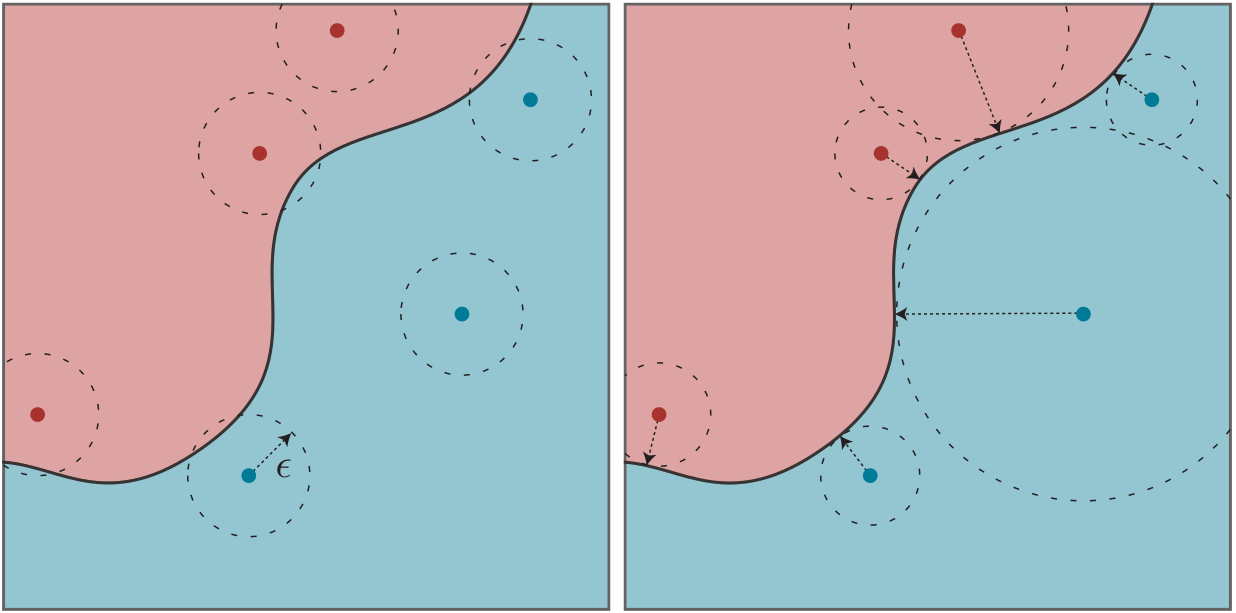
\includegraphics[width=\textwidth/4]{ETH-DS-2020/AML/Resources/adv_examples.png}
\subsection*{Measuring adversarial robustness} 2 equiv. robust defs:
\begin{inparaitem}[$\color{mygreen} \triangleright$]
\item Fraction of $x\in\mathcal{D}$ s.t. $\forall r, ||r||_p \le \epsilon: NN(x) = NN(x+r)$
\item Average norm $||r||_p$ for which $NN(x+r) \ne NN(x)$
\end{inparaitem}

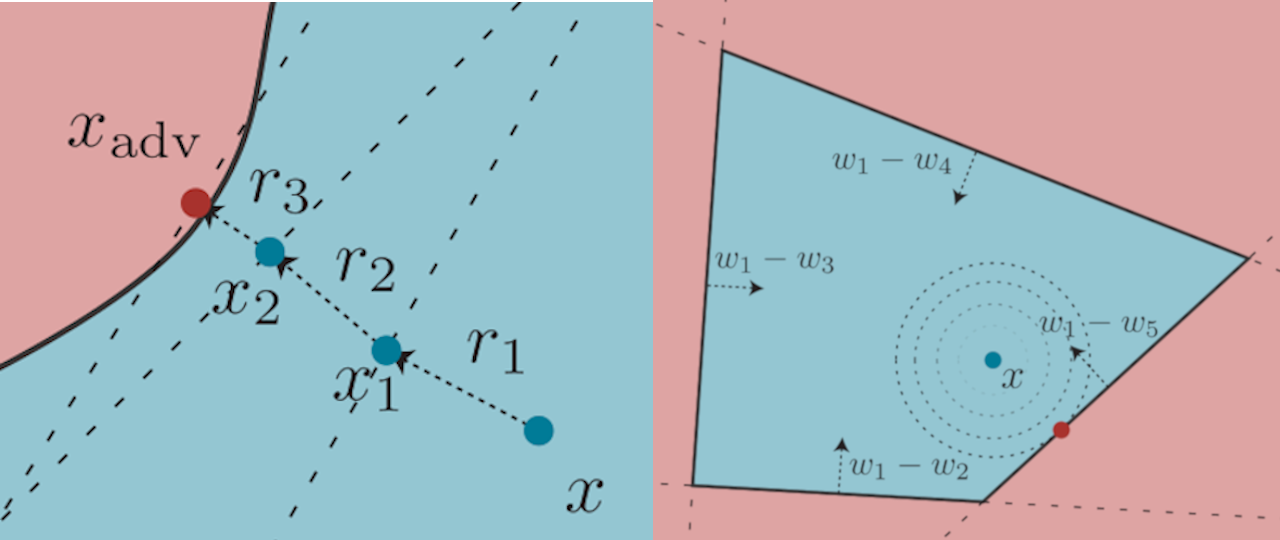
\includegraphics[width=\textwidth/5]{ETH-DS-2020/AML/Resources/adv_examples3.png}
\subsection*{Find adv. perturbation of linear classifier}Given a simple linear classifier $f: \mathbb{R}^d \rightarrow [C],\  f(x) = W^Tx + b$, where $W = [w_1,...,w_c],\ w_i \in \mathbb{R}^d$, $x \in \mathbb{R}^d$ and $f(x) = 1$ the minimal perturbation $r^*$ is:
$r^* = \arg\min_{r_i,\ i\ne 1} ||r_i||_2$ where $r_i = \frac{f_1(x) - f_i(x)}{||w_i - w_1||_2^2}(w_i - w_1)$ (see right image)

\subsection*{Find adv. perturbation of general classifier}Given a general classifier $f: \mathbb{R}^d \rightarrow [C],\ x_0 \in \mathbb{R}^d$ and $f(x_0) = 1$ Idea: Linearize classifier, then iteratively apply solution of linearized classifier problem (see left image). Compute $r^{(i+1)} := \arg\min_{r_k^{(i+1)}} ||r_k^{(i+1)}||$ s.t.\linebreak $(\nabla_x f_1(x_i) - \nabla_x f_k(x_i))^T r_k^{(i+1)} + f_1(x_i) - f_k(x_i)\ <\ 0$\linebreak
and then update $x_{i+1} = x_i + r^{(i+1)}$

\subsection*{Adversarial training} Define robust training procedure:\\ $\min_\theta\max_{||r||_p \le \epsilon}loss(f_\theta(x+r), y)$.\\ Alternately max and min:
\begin{inparaitem}[$\color{mygreen} \triangleright$]
\item Initialize $\theta_0$

\item \term{Maximization step:}

$r^{t+1}(\theta^t) = \arg\max_{||r||_p \le \epsilon} loss(f_{\theta^t}(x+r),y)$\\
\item \term{Minimization step:}

$\theta^{t+1}(r^{t+1}) = \theta^{t} - \eta \nabla_\theta loss(f_{\theta^t}(x+r^{t+1}),y)$
\end{inparaitem}

\subsection*{Projected gradient descent} Solves maxation step in adv training. \term{PGD($n$)} computes $r$ in $n$ steps. For $p = 2$, compute:\\
$\Tilde{r}^{s+1} = r^s + \alpha \nabla_x loss(f_\theta(x + r^s), y)$\\
For $p = \infty$, compute: \\
$\Tilde{r}^{s+1} = r^s + \alpha \cdot sign(\nabla_x loss(f_\theta(x + r^s), y))$\\
Finally, project the resulting perturbation back to the $\epsilon - l_p$ ball:
$r^{s+1} = \Pi_\epsilon^p(\Tilde{r}^{s+1})$\\
A special case is the \term{Fast gradient sign method (FGSM)} which computes only 1 step of PGD (with $p = \infty$) without the projection step. However, this attack is weaker

\subsection*{Undesired side-effects of adversarial training:}
\begin{inparaitem}[$\color{mygreen} \triangleright$]
\item \term{Gradient masking:} the gradient (w.r.t. input) norm becomes too small for training samples ($||\nabla_xf(x)||_p \approx 0$)\\
\item \term{Gradient obfuscation:} The gradient (w.r.t.) input becomes extremely noisy (i.e. spiky) or even undefined
\end{inparaitem}